\apendice{Especificación de Requisitos}

En este apartado se presenta la especificación de requisitos del sistema desarrollado, compuesto por dos addons independientes para Blender: un addon de recopilación de datos y un addon de análisis y visualización de datos.

En primer lugar, se describen los casos de uso más representativos del sistema. Posteriormente, se recogen los objetivos generales, los diagramas que modelan el comportamiento y la arquitectura del sistema, y finalmente el catálogo completo de requisitos funcionales, no funcionales, de interfaz y legales.

\section{Casos de uso}

A continuación, se describen los casos de uso principales del sistema. Las Tablas~\ref{tab:cu1} a~\ref{tab:cu6} recogen de forma estructurada la información esencial de cada caso de uso.

% CU-1
\begin{table}[p]
\centering
\begin{tabularx}{\linewidth}{p{0.25\linewidth} X}
\toprule
\textbf{CU-1} & Registrar creación de objeto en la escena \\
\midrule
\textbf{Versión} & 1.0 \\
\textbf{Autor} & María Molina Goyena \\
\textbf{Requisitos asociados} & RF-01, RF-10 \\
\textbf{Descripción} & Captura automática de la creación de un objeto por parte del usuario, incluyendo propiedades geométricas y posición espacial. \\
\textbf{Precondición} & El addon de recopilación de datos está activado y la sesión de Blender está abierta. \\
\textbf{Acciones} &
\begin{minipage}[t]{\linewidth}
\begin{enumerate}
    \item El usuario crea un nuevo objeto en la escena.
    \item El módulo de captura detecta la acción.
    \item Se extraen las propiedades relevantes del objeto.
    \item Los datos se almacenan en el archivo CSV correspondiente.
\end{enumerate}
\end{minipage} \\
\textbf{Postcondición} & El evento queda registrado y disponible para su análisis posterior. \\
\textbf{Excepciones} & Error en la captura debido a conflicto con otro addon o fallo interno de Blender. \\
\textbf{Importancia} & Alta \\
\bottomrule
\end{tabularx}
\caption{CU-1: Registro de creación de objetos.}
\label{tab:cu1}
\end{table}

% CU-2
\begin{table}[p]
\centering
\begin{tabularx}{\linewidth}{p{0.25\linewidth} X}
\toprule
\textbf{CU-2} & Registrar modificaciones de geometría de un objeto \\
\midrule
\textbf{Versión} & 1.0 \\
\textbf{Autor} & María Molina Goyena \\
\textbf{Requisitos asociados} & RF-02, RF-10 \\
\textbf{Descripción} & Detecta cambios en la geometría de los objetos, incluyendo vértices, aristas y caras, y registra las modificaciones realizadas. \\
\textbf{Precondición} & El addon de recopilación de datos está activo y el objeto existe en la escena. \\
\textbf{Acciones} &
\begin{minipage}[t]{\linewidth}
\begin{enumerate}
    \item El usuario realiza modificaciones en el objeto.
    \item El sistema detecta los cambios geométricos mediante handlers de Blender.
    \item Se registran las propiedades previas y actuales del objeto.
    \item Los datos se almacenan para su análisis temporal y estructural posterior.
\end{enumerate}
\end{minipage} \\
\textbf{Postcondición} & La modificación queda registrada con información suficiente para analizar los cambios relevantes. \\
\textbf{Excepciones} & Error en la captura si la malla es demasiado compleja o existe conflicto con otro addon. \\
\textbf{Importancia} & Alta \\
\bottomrule
\end{tabularx}
\caption{CU-2: Registro de modificaciones de geometría.}
\label{tab:cu2}
\end{table}

% CU-3
\begin{table}[p]
\centering
\begin{tabularx}{\linewidth}{p{0.25\linewidth} X}
\toprule
\textbf{CU-3} & Registrar cambio de modo de edición \\
\midrule
\textbf{Versión} & 1.0 \\
\textbf{Autor} & María Molina Goyena \\
\textbf{Requisitos asociados} & RF-03, RF-10 \\
\textbf{Descripción} & Detecta y registra los cambios de modo de trabajo en Blender, especialmente entre \textit{Object Mode} y \textit{Edit Mode}. \\
\textbf{Precondición} & El addon de recopilación de datos está activo. \\
\textbf{Acciones} &
\begin{minipage}[t]{\linewidth}
\begin{enumerate}
    \item El usuario cambia el modo de edición de un objeto.
    \item El sistema detecta el cambio mediante handlers de Blender.
    \item Se registra el modo anterior, el modo actual y el objeto afectado.
\end{enumerate}
\end{minipage} \\
\textbf{Postcondición} & El cambio de modo queda registrado con su marca temporal correspondiente. \\
\textbf{Excepciones} & Fallo en la captura si la escena está bloqueada o el objeto ya no existe. \\
\textbf{Importancia} & Media \\
\bottomrule
\end{tabularx}
\caption{CU-3: Registro de cambios de modo.}
\label{tab:cu3}
\end{table}

% CU-4
\begin{table}[p]
\centering
\begin{tabularx}{\linewidth}{p{0.25\linewidth} X}
\toprule
\textbf{CU-4} & Registrar eliminación de objeto \\
\midrule
\textbf{Versión} & 1.0 \\
\textbf{Autor} & María Molina Goyena \\
\textbf{Requisitos asociados} & RF-04, RF-10 \\
\textbf{Descripción} & Registra la eliminación de un objeto de la escena, almacenando sus propiedades relevantes antes de su desaparición. \\
\textbf{Precondición} & El addon de recopilación de datos está activo y el objeto existe en la escena. \\
\textbf{Acciones} &
\begin{minipage}[t]{\linewidth}
\begin{enumerate}
    \item El usuario elimina un objeto.
    \item El addon detecta la eliminación mediante handlers.
    \item Se registran propiedades clave del objeto eliminado y la marca temporal de la acción.
\end{enumerate}
\end{minipage} \\
\textbf{Postcondición} & La eliminación queda registrada para su análisis histórico posterior. \\
\textbf{Excepciones} & Fallo si la escena está corrupta o existe conflicto con otro addon. \\
\textbf{Importancia} & Alta \\
\bottomrule
\end{tabularx}
\caption{CU-4: Registro de eliminación de objetos.}
\label{tab:cu4}
\end{table}

% CU-5
\begin{table}[p]
\centering
\begin{tabularx}{\linewidth}{p{0.25\linewidth} X}
\toprule
\textbf{CU-5} & Visualizar métricas de modelado \\
\midrule
\textbf{Versión} & 1.0 \\
\textbf{Autor} & María Molina Goyena \\
\textbf{Requisitos asociados} & RF-05, RF-07 \\
\textbf{Descripción} & Permite consultar métricas temporales, espaciales y estadísticas obtenidas a partir de la sesión de modelado registrada. \\
\textbf{Precondición} & El addon de análisis tiene acceso a los archivos CSV generados por el addon de recopilación. \\
\textbf{Acciones} &
\begin{minipage}[t]{\linewidth}
\begin{enumerate}
    \item El usuario abre el panel de métricas.
    \item El addon carga los datos registrados.
    \item El addon calcula las métricas correspondientes.
    \item Se muestran gráficas y resúmenes visuales filtrables por objeto, evento o rango temporal.
\end{enumerate}
\end{minipage} \\
\textbf{Postcondición} & Las métricas quedan visibles para el usuario. \\
\textbf{Excepciones} & Datos incompletos, corruptos o error en el cálculo de métricas. \\
\textbf{Importancia} & Alta \\
\bottomrule
\end{tabularx}
\caption{CU-5: Visualización de métricas.}
\label{tab:cu5}
\end{table}

% CU-6
\begin{table}[p]
\centering
\begin{tabularx}{\linewidth}{p{0.25\linewidth} X}
\toprule
\textbf{CU-6} & Exportar datos a archivo externo \\
\midrule
\textbf{Versión} & 1.0 \\
\textbf{Autor} & María Molina Goyena \\
\textbf{Requisitos asociados} & RF-06 \\
\textbf{Descripción} & Permite exportar los datos registrados para su consulta o tratamiento externo. \\
\textbf{Precondición} & Existen datos previamente registrados y el addon de análisis está activo. \\
\textbf{Acciones} &
\begin{minipage}[t]{\linewidth}
\begin{enumerate}
    \item El usuario selecciona la opción de exportación.
    \item El addon prepara los registros almacenados.
    \item El archivo se guarda en la ubicación indicada por el usuario.
\end{enumerate}
\end{minipage} \\
\textbf{Postcondición} & Los datos quedan disponibles para análisis externo. \\
\textbf{Excepciones} & Error de escritura o permisos insuficientes en la ruta de destino. \\
\textbf{Importancia} & Media \\
\bottomrule
\end{tabularx}
\caption{CU-6: Exportación de datos.}
\label{tab:cu6}
\end{table}

\clearpage

\section{Objetivos generales}

A partir de los casos de uso descritos, se establecen los objetivos generales que debe satisfacer el sistema:

\begin{itemize}
    \item Registrar de manera precisa los eventos relevantes producidos durante el modelado 3D.
    \item Permitir el análisis estadístico y la visualización de los datos recopilados.
    \item Garantizar la persistencia, integridad y trazabilidad de los datos entre sesiones.
    \item Proporcionar una interfaz clara y segura para la interacción con ambos addons.
    \item Cumplir con la normativa legal y ética relativa a la protección de datos y al uso de software libre.
\end{itemize}

\section{Diagramas del sistema}

Con el fin de complementar la descripción textual del sistema, se incluyen a continuación varios diagramas que representan sus funcionalidades, flujo de trabajo, secuencia de interacción y arquitectura general.

La Figura~\ref{fig:casos_uso} muestra el diagrama UML de casos de uso. En él se representa al usuario como actor principal y se identifican las funcionalidades más importantes del sistema.

\begin{figure}[H]
    \centering
    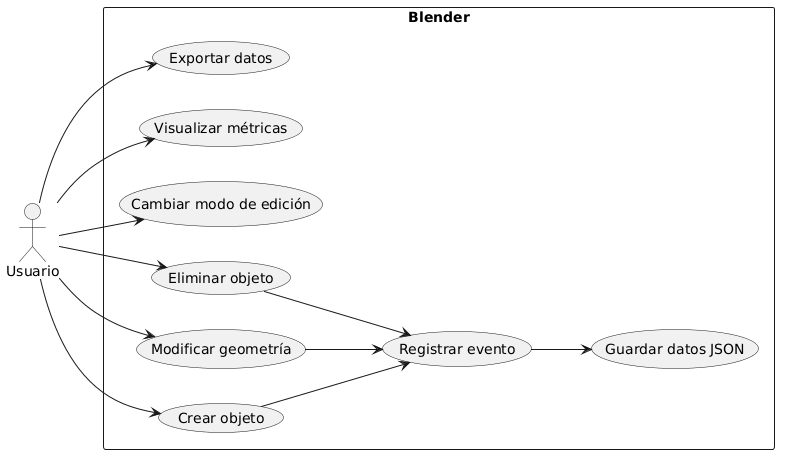
\includegraphics[width=0.8\textwidth]{diagramas/uml_casos_uso.png}
    \caption{Diagrama UML de casos de uso del sistema.}
    \label{fig:casos_uso}
\end{figure}

La Figura~\ref{fig:flujo} representa el flujo general de procesamiento del sistema, desde la interacción inicial del usuario con Blender hasta la visualización de métricas.

\begin{figure}[H]
    \centering
    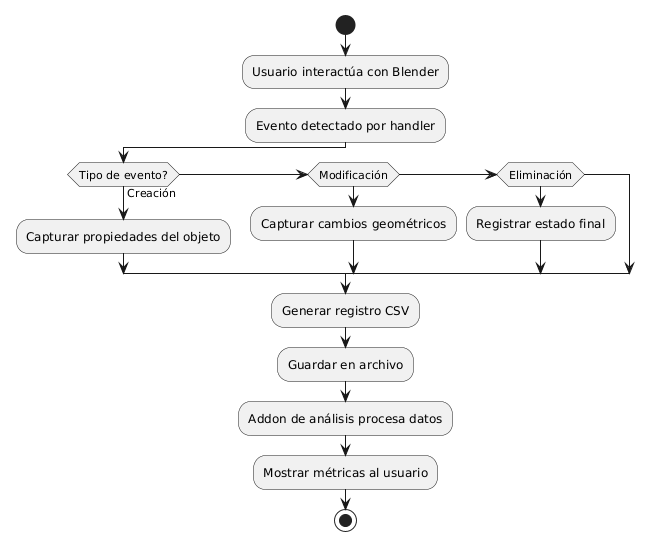
\includegraphics[width=0.8\textwidth]{diagramas/flujo.png}
    \caption{Diagrama de flujo de captura, registro y análisis de eventos.}
    \label{fig:flujo}
\end{figure}

La Figura~\ref{fig:arquitectura} muestra una visión general del sistema, basada en los dos addons desarrollados.

\begin{figure}[H]
    \centering
    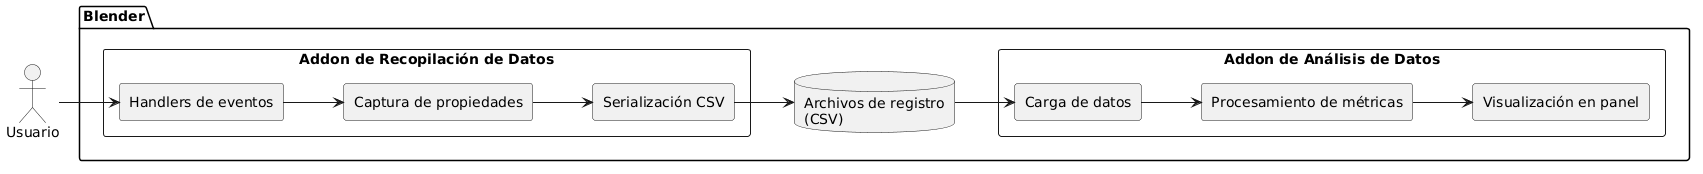
\includegraphics[width=0.85\textwidth]{diagramas/arquitectura.png}
    \caption{Arquitectura del sistema basada en los dos addons: recopilación de datos y análisis de métricas.}
    \label{fig:arquitectura}
\end{figure}

\section{Catálogo de requisitos}

\subsection{Requisitos funcionales (RF)}

\begin{itemize}
    \item RF-01: Registrar la creación de objetos.
    \item RF-02: Registrar modificaciones de geometría.
    \item RF-03: Detectar cambios de modo de edición.
    \item RF-04: Registrar la eliminación de objetos.
    \item RF-05: Visualizar métricas de modelado.
    \item RF-06: Exportar datos a archivo externo.
    \item RF-07: Filtrar métricas por objeto, evento o tiempo.
    \item RF-08: Notificar errores en los datos o en su procesamiento.
    \item RF-09: Activar y desactivar la captura desde la interfaz de usuario.
    \item RF-10: Registrar marcas temporales precisas en cada evento.
\end{itemize}

\subsection{Requisitos no funcionales (RNF)}

\begin{itemize}
    \item RNF-01: Eficiencia en la captura de eventos.
    \item RNF-02: Soporte de múltiples objetos y cambios complejos.
    \item RNF-03: Persistencia de datos ante cierres inesperados.
    \item RNF-04: Interfaz clara e intuitiva.
    \item RNF-05: Código mantenible y modular.
\end{itemize}

\subsection{Requisitos de interfaz de usuario (RIU)}

\begin{itemize}
    \item RIU-01: Panel de control de captura.
    \item RIU-02: Panel de métricas con gráficas y tablas.
    \item RIU-03: Configuración de exportación de datos.
    \item RIU-04: Alertas de errores y estados del sistema.
\end{itemize}

\subsection{Requisitos legales y éticos (RLE)}

\begin{itemize}
    \item RLE-01: Cumplimiento de la normativa de protección de datos.
    \item RLE-02: Consentimiento explícito del usuario para la recopilación de datos.
    \item RLE-03: Uso de software libre respetando las licencias aplicables.
\end{itemize}

\section{Especificación de requisitos}

Una vez definido el catálogo general, la Tabla~\ref{tab:requisitos} recoge de forma consolidada la especificación completa de requisitos del sistema.

\begin{table}[p]
\centering
\begin{tabular}{l p{6.2cm} p{2.7cm} p{1.5cm} p{2.8cm}}
\toprule
\textbf{ID} & \textbf{Descripción} & \textbf{Addon} & \textbf{Prioridad} & \textbf{Verificación} \\
\midrule
RF-01 & Registrar creación de objetos & Recopilación & Alta & CU-1 \\
RF-02 & Registrar modificaciones de geometría & Recopilación & Alta & CU-2 \\
RF-03 & Detectar cambios de modo de edición & Recopilación & Media & CU-3 \\
RF-04 & Registrar eliminación de objetos & Recopilación & Alta & CU-4 \\
RF-05 & Visualizar métricas de modelado & Análisis & Alta & CU-5 \\
RF-06 & Exportar datos & Análisis & Media & CU-6 \\
RF-07 & Filtrar métricas & Análisis & Media & CU-5 \\
RF-08 & Notificar errores en datos & Ambos & Media & Panel/Logs \\
RF-09 & Activar o desactivar captura desde la interfaz & Recopilación & Alta & Panel de control \\
RF-10 & Registrar marcas temporales precisas & Recopilación & Alta & Logs internos \\
RNF-01 & Eficiencia en captura de eventos & Ambos & Alta & Pruebas de rendimiento \\
RNF-02 & Soporte de múltiples objetos & Ambos & Alta & Pruebas de estrés \\
RNF-03 & Persistencia ante cierres inesperados & Ambos & Alta & Pruebas de reinicio \\
RNF-04 & Interfaz clara e intuitiva & Ambos & Media & Evaluación de usabilidad \\
RNF-05 & Código mantenible y modular & Ambos & Media & Revisión de código \\
RIU-01 & Panel de control de captura & Recopilación & Alta & Prueba de interfaz \\
RIU-02 & Panel de métricas & Análisis & Alta & Prueba de interfaz \\
RIU-03 & Configuración de exportación & Análisis & Media & Prueba de interfaz \\
RIU-04 & Alertas de errores & Ambos & Media & Prueba de interfaz \\
RLE-01 & Cumplimiento de normativa de protección de datos & Ambos & Alta & Documentación legal \\
RLE-02 & Consentimiento explícito del usuario & Recopilación & Alta & Confirmación del usuario \\
RLE-03 & Uso de software libre respetando licencias & Ambos & Media & Licencias verificadas \\
\bottomrule
\end{tabular}
\caption{Especificación completa de requisitos.}
\label{tab:requisitos}
\end{table}